\chapter{Theoretical foundation}
\label{sec:theory}

\section{Sequential decision making}

Lane keeping of a car is a sequential decision making task. Every steering action that is performed directly influences the choice of the best succeeding steering actions. \Glspl{mdp} are well suited and widely used to model sequential decision making tasks. An \gls{mdp} is a discrete time framework for a decision maker, the agent, to interact with an environment. At every time step, the environment is in a certain state, fully observable by the agent. The agent interacts with the environment by performing an action that determines the next state of the environment. The underlying assumption, the Markov property, is that the next state of the environment only depends on its current state and the agent's action. The transition to a succeeding state after an action has been performed does not need to be deterministic but can be probabilistic, accounting for randomness in the environment. After performing an action, the agent receives a numerical reward (also called return). The agent's goal is to maximize the cumulative reward it receives over time. An action that leads to a high immediate return is not optimal if another action leads to a higher cumulative reward in the long run. Thus, the agent needs to find an optimal policy that decides the best action to take in every state. In case the state transition probabilities are known to the agent, the optimal policy can be found using model-based techniques such as value or policy iteration. If the transition model is unknown, model-free reinforcement learning can be applied to learn an optimal policy. % TODO: Add source

\begin{figure}[htbp]
    \centering
    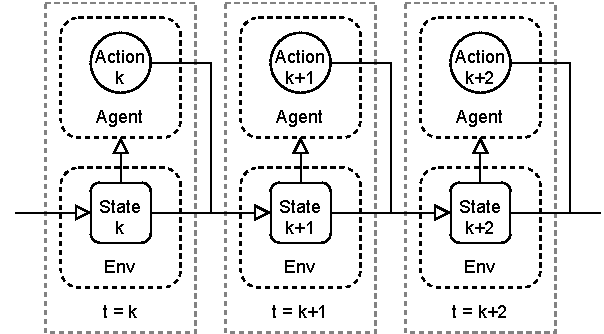
\includegraphics[width=0.75\textwidth]{figures/MDP.pdf}
    \caption{\acrfull{mdp}}
\end{figure}

Assisting a human driver in the lane keeping task is essentially a sequential decision making task as well. However, the agent that is assisting the human driver does not know about the driver's internal psychological state, and therefore her attention. A distracted driver may steer poorly and needs assistance. But how can the agent tell whether the driver is distracted? Reading the driver's mind is not feasible and even if it were, it would be too invasive for this task. Instead, the agent needs to estimate the driver's internal state in order to act adequately. A \Gls{pomdp} is a generalization of an MDP that allows to plan under uncertainty. Even without observing the full state of the agent's environment, of which the driver is part of, a POMDP allows the agent to estimate the environment's true state using the partial information it observes. A POMDP serves as the foundation of this thesis. The lane keeping assistance problem this thesis aims to solve can be defined as a POMDP. First, a formal definition is needed.

\section{Partially observable Markov decision process (POMDP)}
\label{def:pomdp}
% See POMDP Model from (POMDP algorithm) Online Planning Algorithms for POMDPs

The POMDP generalizes the MDP for planning under uncertainty. The environment's true state is unknown to the agent. It has to rely on observations with partial information about the environment's true state to choose its actions. \cite{pomdp-definition} define a POMDP as a tuple $(S, A, T, R, O, Z)$, where:
\begin{itemize}
    \item $S$ is the set of all possible states $s \in S$ of the environment. A state describes the environment at a time point. It must not be an all-encompassing description but must include all relevant information to make decisions. The state is hidden from the agent. This is the main difference to an MDP.
    \item $A$ is the set of all possible actions $a \in A$ the agent can perform in the environment.
    \item $T : S \times A \times S \rightarrow [0,1]$ defines the conditional state transition probabilities. $T(s,a,s') = Pr(s' | s, a)$ constitutes the probability of transitioning to state $s'$ after performing action $a$ in state $s$.
    \item $R : S \times A \rightarrow \R$ is the reward function providing the agent with a reward of $R(s,a)$ after performing action $a$ in state $s$.
    \item $O$ is the set of all possible observations $o \in O$. Observations are the agent's source of information about the environment, enabling the agent to estimate the environment's state.
    \item $Z : S \times A \times O \rightarrow [0,1]$ defines the conditional observation probabilities. $Z(s', a, o) = Pr(o | s', a)$ represents the probability of receiving observation $o$ at state $s'$ after performing action $a$ in the previous state. 
\end{itemize}

At any time, the environment is in some state $s$. Unlike in the case of an MDP, the agent cannot directly observe the environment's state. Instead, the agent receives an observation $o$ that provides partial information about the current state. The agent uses the observations it perceives over time to estimate the true state of the environment in order to choose adequate actions. At any time step $t$, it has to take into account the complete history $h_t$ of actions and observations until $t$:

\begin{equation}
    h_t = \{a_0,o_1,...,o_{t-1},a_{t-1},o_t\}
\end{equation}

Keeping a collection of all past observations and actions is very memory expensive. A less memory demanding alternative is to only keep a probability distribution over the states at every step, called a belief $b$. $b(s,h)$ denotes the probability of being in state $s$ given history $h$. 

\begin{equation}
    b_t(s,h) = Pr(s_t = s|h_t = h)
\end{equation}

The belief is a sufficient statistic for the agent to form a decision about its next action \parencite{pomdp-belief}. Thus, only the belief needs to be kept and can be recursively updated whenever an action is performed and a new observation arises. The agent starts with an initial belief $b_0$ about the initial state of the environment. At every subsequent time step, the new belief $b'$ can be recursively calculated based on the previous belief $b$, the last action $a$ and the current observation $o$. The previous belief can then be discarded as the history it represents is no longer up-to-date. For an exact update of the belief one can apply the Bayes theorem:

\begin{equation}
    \label{eq:bayes_update}
    \begin{split}
        b'(s') & = Pr(s' | o, a , b) \\
               & = \frac{Pr(o | s', a, b)Pr(s' | a,b)}{Pr(o| a, b)} \\
               & = \frac{Pr(o | s', a)\sum_{s \in S}Pr(s' | a, b, s)Pr(s| a, b)}{Pr(o| a, b)} \\
               & = \frac{Z(s', a, o)\sum_{s \in S}T(s, a, b)b(s)}{Pr(o | a, b)}
    \end{split}
\end{equation}

The agent chooses its actions based on its belief according to its policy $\pi$. The agent's policy defines the action to choose at any given belief state. It describes the strategy for every possible situation the agent can encounter. Solving a \gls{pomdp} consists in finding an optimal policy $\pi^*$ that maximizes the the cumulative reward obtained over some time horizon $N$ starting from initial belief $b_0$ using a discount factor $0 \leq \lambda \leq 1$:

\begin{equation}
    \pi^* = argmax_{\pi}~E\left[ \sum_{t=0}^{N} \sum_{s \in S}b_t(s) \sum_{a \in A} \lambda^t R(s,a) \pi(b_t,a) | b_0\right]
\end{equation}

% Value function
The return that is gained by following a policy $\pi$ from a certain belief $b$ can be obtained with the value function $V^\pi(b)$:

\begin{equation}
    V^\pi(b) = \sum_{a \in A} \pi(b,a) \left[ \sum_{s \in S} b(s) R(s,a) + \lambda \sum_{o \in O} Pr(o | b, a) V^\pi(b')\right]
\end{equation}

The optimal policy $\pi^*$ maximizes $V^\pi(b_0)$. For any POMDP there exists at least one optimal policy.

\section{Key challenges}




% As we have discussed above, POMDPs are affected by the curse of history; their computational complexity grows exponentially with the planning horizon. A second challenge, shared with MDPs, is the curse of dimensionality. The size of the state space grows exponentially with the number of state variables. POMDPs, in particular, need to plan on a (|S| − 1)-dimensional continuous belief space. If we were to discretize this belief space, the number of possible beliefs would grow exponentially with the number of states. In this subsection, we present some of the existing literature to overcome these challenges and to solve POMDPs approximately. We focus here on offline approaches, where the optimal action is approximately calculated for all possible beliefs before any execution takes place. The next subsection will cover online approaches, which interleave execution and planning. The main advantage of offline methods is a faster policy execution, since no further planning is required. Approximate solution methods for POMDPs can be classified into value-based and policy-based.


\subsection{Curse of dimensionality and curse of history}

Computing an optimal policy for a POMDP is challenging for two distinct but interdependent reasons \parencite{pomdp_curses}. On the one hand, there is the so-called curse of history: Finding an optimal policy is like searching through the space of possible action-observation histories. The number of distinct histories grows exponentially with the size of the time horizon. Therefore, planning further into the future increases the computation complexity exponentially. While finding an optimal policy can be relatively easy for short histories, it becomes computationally infeasible for larger time horizons. On the other hand, there is the curse of dimensionality: The belief space is a $|S|$-dimensional. Therefore, the size of the belief space, representing the number of states in a POMDP, grows exponentially with $|S|$.

The task of finding an optimal policy for a finite POMDP is PSPACE-complete \parencite{pomdp_complex}. Therefore, solving POMDP to optimality is computationally infeasible with a large state space or time horizon. For this reason, approximate algorithms are often applied. 

\subsection{Unknown transition and observation probabilities}

For many problems, it is difficult or impossible to know the probability distributions $T$ or $Z$ explicitly. This is also the case for the shared control lane keeping scenario assessed in this thesis. Neither the transition probabilities, nor the observation probabilities are known a priori. The belief update method using Bayes' theorem presented in Equation \ref{eq:bayes_update} is not computable without knowing the probabily distributions explicitly. However, exact updates are too complex for problems with a large state space in any case \parencite{pomcp}. Some solution approaches circumvent the problem of unknown transition and observation probability distributions by only requiring a generative model that can sample state and observation transitions. A generative model can stochastically generate a successor state, reward, and observation, given the current state and action. Thereby, it implicitly defines the transition and observation probabilities, even if they are not explicitly known. The generative model used in this thesis is described in detail in Section \ref{sec:gen_model}.

% \subsection{Exploration versus exploitation}
% TODO: Move?

% \section{Algorithms to solve POMDP}
\section{Algorithms to aproximately solve large POMDP}

% POMCP - bayes belief rule only for small state spaces (see Monte-Carlo Belief State Updates)

% Planning: Computational process that takes a model as input and produces or improves a policy for interacting with the modeled environment.
% Learning: Whereas planning methods use simulated experience generated by a model, learning methods use real experience generated by the environment.

\subsection{Offline and online solvers}

% Generally, POMDP solver can be classified into two categories, online solver and offline solver. Since the traffic environments are nondeterministic and the dimension of the motion planning problem for autonomous driving is quite large, online solver behaves much better to duel with the uncertain environment and huge observation space [16].

\begin{figure}[htbp]
    \centering
    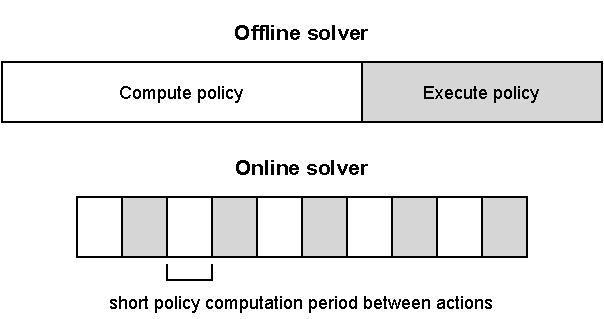
\includegraphics[width=0.6\textwidth]{figures/online-offline.pdf}
    \caption{Comparison of offline and online solving procedure}
\end{figure}

% TODO: REFINE

\noindent
There are two general approaches to solve POMDP: offline and online. Online solvers compute the optimal policy prior to execution for all possible future scenarios. Their advantage is that once the policy is found, its the application does only have a very minimal, negligible time overhead. However, offline planning is hard to scale to complex problems as the number of possible future scenarios grows exponentially with the size of the time horizon (curse of history). Furthermore, while the performance for small to medium sized POMDP can be quite good, computing the policy may take a very long time, and even small changes in the dynamics of the environment require a full recomputation \parencite{online_pomdp}. Online solvers interleave planning and plan execution. At every time step, only the current belief is considered to compute the next optimal action by searching ahead until a certain depth is reached. On the one hand, the scalability is greatly increased. On the other hand, sufficiently more online computation than with offline planning is required. The amount of available online planning time at each time step limits the performance. 

Because the state space 

% TODO: Give examples for good offline solvers

% TODO: Online solvers overview
% See (POMDP, POMCP, Thesis) Towards Human-Like Prediction and Decision-Makingfor Automated Vehicles in Highway Scenarios
% Generally, a search tree rooted at the current belief is constructed
% by considering all possible actions and observations; the tree alternates layers with belief nodes and with action nodes (Figure 2.2a). The goal is to “smartly” explore the tree so that the value at the current belief is quickly and correctly estimated. Online POMDP algorithms interleave search steps with execution steps. As a consequence, the time available for planning is usually shorter than for offline approaches. Because of this, some online approaches leverage policies computed offline in order to speed up the search. After a search step is completed, the agent executes the best action from the current belief and receives an observation from the environment; the search procedure continues then from the new belief. Depending on the method used to explore the search tree, online POMDP algorithms are classified into three main groups: branch-and-bound pruning, heuristic search, and Monte Carlo sampling (Ross et al.,
% 2008).

\subsection{Monte Carlo tree search solvers}

% See Monte Carlo Tree Search in (POMDP, Continuous, POMCPOW, POMCP-DOW, DPW, Thesis) SAFETY AND EFFICIENCY IN AUTONOMOUS VEHICLES THROUGH PLANNING WITH UNCERTAINTY

% General purpose online algorithms for POMDPs have also been proposed. These algorithms are mostly derivatives of the MCTS algorithm for MDPs (Section 1.2.6). A conceptually straightforward way to solve a POMDP using MCTS is to apply it to the corresponding belief MDP. Indeed, many tree search techniques have been applied to POMDP problems in this way [76]. However, when the Bayesian belief update is used, this approach is computationally expensive.

% A major improvement in efficiency came with the introduction of the partially observable Monte Carlo planning (POMCP) algorithm [87]. It is based on UCT, but can tackle problems many times larger than its predecessors because it uses state trajectory simulations, rather than full belief trajectories, to build the tree. Each node in the POMCP tree corresponds to an action- or observation-terminated history. At each iteration, a state is sampled from the current belief and simulated through the nodes that match the history as it is generated. Thus, the belief at each observation-terminated history node is effectively represented by the collection of states for the appropriate time step in the trajectories that match the history. This is similar to using a rejection sampling unweighted particle filter. It should be noted that when this thesis uses the term POMCP, it refers only to the UCT-based decision-making algorithm called PO-UCT by Silver, Huang, Maddison, et al. [87] and not to the belief update scheme that re-uses simulations from the planning stage.Determinized sparse partially observable tree (DESPOT) is a similar approach that attempts to achieve better performance by analyzing only a small number of random outcomes in the tree [92]. Additionally, an algorithm called adaptive belief tree (ABT) was designed specifically to accommodate changes in the environment without having to replan from scratch [57]. Some very recent methods, e.g. QMDP-Net [46], have attempted to solve POMDPs by training recurrent neural networks.


% expanding the search tree fully over a large set of observations is infeasible except for shallow depths. In such cases, a better alternative may be to sample a subset of observations at each expansion and only consider beliefs reached by these sampled observations. This reduces the branching factor of the search and allows for deeper search within a set planning time. This is the strategy employed by Monte Carlo algorithms.


% POMCP
% Recently an online POMDP planning algorithm called POMCP has successfully scaled up to very 
% large POMDPs [18]. POMCP, which is based on Monte Carlo tree search, tries to break the two
% curses by sampling states from the current belief and sampling histories with a black-box simula-
% tor. It uses the UCT algorithm [9] to control the exploration-exploitation trade-off during the online
% lookahead search. However, UCT is sometimes overly greedy and suffers the worst-case perfor-
% mance of Ω(exp(exp(...exp(1) ...)))1 samples to find a sufficiently good action [4].

% DESPOT
% This paper presents a new algorithm for online POMDP planning. It enjoys the same strengths
% as POMCP—breaking the two curses through sampling—but avoids POMCP’s extremely poor
% worst-case behavior by evaluating policies on a small number of sampled scenarios [13]. In each
% planning step, the algorithm searches for a good policy derived from a Determinized Sparse Par-
% tially Observable Tree (DESPOT) for the current belief, and executes the policy for one step. A
% DESPOT summarizes the execution of all policies under K sampled scenarios. It is structurally
% similar to a standard belief tree, but contains only belief nodes reachable under the K scenarios

% The general concept of online POMDP planning is that the solver computes the next optimal
% action based on the current belief state by searching in a certain depth ahead. DESPOT
% adopts this concept and improves the computational efficiency by shrinking the observation
% space.

% In order to do an efficient search in a large and deep belief tree, it is pruned and transferred 
% to Determinized Sparse Partially Observable Tree. The construction of DESPOT is sampled by the 
% K scenarios, which are shown as dots in the figure. A scenario is a determinized simulation 
% trajectory from the root of the tree. Each Q-state maintains the scenarios from its ancestor.
% And the observation is determinized by the randomly sampled scenarios. Each depth of the tree 
% can be regarded as one time-step forward simulation of the model. Thus the observation space is 
% sampled by the scenarios, but the action space is kept as its original size.





% Requirement of observation probabilities for other solvers
Other solvers have build upon the principle from POMCP of using Monte Carlo tree search for POMDP planning. 
Notably, there are DESPOT, POMCPOW, ... TODO ...
They all have an important requirement in common: The observation probabilities need to be known to the solver. Thereby, particles that are added to the belief can be weighed by how likely their associated observation is at the current belief state after performing a certain action in the prior state. However, the observation probabilities are essentially unknown in our assisted driving scenario. 

% TODO ...